\documentclass[conference]{IEEEtran}
\IEEEoverridecommandlockouts

\usepackage{cite}
\usepackage{amsmath,amssymb,amsfonts}
\usepackage{graphicx}
\usepackage{textcomp}
\usepackage{xcolor}
\usepackage{booktabs}
\usepackage{multirow}
\usepackage{url}
\usepackage{algorithm}
\usepackage{algorithmic}
\usepackage{tikz}
\usetikzlibrary{arrows.meta, positioning, calc}
\usepackage{pgfplots}
\pgfplotsset{compat=1.18}
% Enable clickable hyperlinks for in-text citations, figures, tables, and equations
\usepackage[colorlinks=true, linkcolor=blue, citecolor=blue, urlcolor=blue]{hyperref}

% Color definitions for publication-quality TikZ and pgfplots
\definecolor{origblue}{RGB}{30, 58, 138}
\definecolor{smoteorange}{RGB}{217, 119, 6}
\definecolor{adasynpurple}{RGB}{124, 58, 237}
\definecolor{tmggreen}{RGB}{15, 118, 110}
\definecolor{cmblue}{RGB}{27, 79, 138}
\definecolor{cmwhite}{RGB}{245, 247, 250}

% IEEEtran float tuning: allows dense column packing without artificial whitespace
\renewcommand{\topfraction}{0.95}
\renewcommand{\bottomfraction}{0.85}
\renewcommand{\textfraction}{0.05}
\renewcommand{\floatpagefraction}{0.85}
\renewcommand{\dbltopfraction}{0.95}
\renewcommand{\dblfloatpagefraction}{0.85}
\setlength{\textfloatsep}{8pt plus 2pt minus 2pt}
\setlength{\floatsep}{8pt plus 2pt minus 2pt}
\setlength{\intextsep}{8pt plus 2pt minus 2pt}
\setlength{\dbltextfloatsep}{8pt plus 2pt minus 2pt}
\setlength{\dblfloatsep}{8pt plus 2pt minus 2pt}

\def\BibTeX{{\rm B\kern-.05em{\sc i\kern-.025em b}\kern-.08em
    T\kern-.1667em\lower.7ex\hbox{E}\kern-.125emX}}

\begin{document}

\title{TMG-GAN: A Multi-Generator Adversarial Framework for Imbalanced Network Intrusion Detection}

\author{
\IEEEauthorblockN{Rishabh Gupta\IEEEauthorrefmark{1}, Uday Kharatmol\IEEEauthorrefmark{2}, Krishna Bhatt\IEEEauthorrefmark{3}, Someshwar Sahu\IEEEauthorrefmark{4}, Ameer Hamza Khan\IEEEauthorrefmark{5}, and Nagendra Yadav\IEEEauthorrefmark{6}}
\IEEEauthorblockA{Department of Computer Science and Engineering\\
Indian Institute of Information Technology Vadodara\\
Gandhinagar, Gujarat, India\\
Email: \IEEEauthorrefmark{1}rishabh\_gupta@iiitvadodara.ac.in,
\IEEEauthorrefmark{2}20261603031@iiitvadodara.ac.in,
\IEEEauthorrefmark{3}20261603014@iiitvadodara.ac.in,\\
\IEEEauthorrefmark{4}202451155@iiitvadodara.ac.in, \IEEEauthorrefmark{5}202451015@iiitvadodara.ac.in, \IEEEauthorrefmark{6}202451112@iiitvadodara.ac.in}
}

\maketitle

\begin{abstract}
Network intrusion detection systems (NIDSs) must identify rare malicious traffic hidden within high-volume normal network traffic. In benchmark datasets such as CICIDS2017, severe threats such as Web attacks (1,476 flows, 1.02\%) and bot activity (857 flows, 0.59\%) make up a small fraction of the 145,149 training flows, making them difficult for standard deep neural networks (DNNs) to detect. Resampling methods such as the Synthetic Minority Over-sampling Technique (SMOTE) and Adaptive Synthetic Sampling (ADASYN) interpolate linearly between nearest neighbors, potentially creating unrealistic boundary flows that trigger excess false alarms. This study evaluates a multi-generator conditional generative adversarial network (TMG-GAN) framework that reshapes 78 network statistics into $13 \times 6$ spatial feature matrices, trains dedicated generators for each of the five minority classes, and stabilizes training through spectral normalization. Before downstream classifier training, candidate samples are filtered using both an auxiliary-classifier confidence threshold ($\tau_{\text{conf}} = 0.50$) and a discriminator-based realism criterion ($\tau_D = 0.0$). The filtering process achieves a 98.10\% acceptance rate and retains 13,059 synthetic flows per minority class, producing a balanced training set of 210,444 flows. Across three random seeds and 710,976 held-out test flows, TMG-GAN achieves a macro F1-score of $0.7940 \pm 0.0237$ and macro precision of $73.41\% \pm 3.28\%$, while reducing the benign false-positive rate (FPR) to $2.3088\% \pm 0.2161\%$. On the 621,677 benign test flows, this corresponds to 2,038 fewer false alarms than SMOTE (14,353 versus 16,391) and 3,877 fewer false alarms than ADASYN (14,353 versus 18,230).
\end{abstract}

\begin{IEEEkeywords}
Network Intrusion Detection, Generative Adversarial Networks, Class Imbalance, False-Positive Rate, Deep Learning, CICIDS2017.
\end{IEEEkeywords}

\section{Introduction}

Modern enterprise infrastructure generates millions of network flows every second, making network intrusion detection an increasingly challenging task. Although deep neural networks (DNNs) achieve high nominal classification accuracy, real-world network environments often exhibit extreme class imbalance, where normal traffic significantly outweighs malicious activities~\cite{sharafaldin2018toward}. In production environments, approximately 90\%--99\% of network flows may represent normal activities, while sophisticated attacks, such as infiltration bots, web exploits, and brute-force intrusions, account for only a small fraction of the overall traffic. This imbalance creates a significant challenge for learning-based intrusion detection systems. When standard cross-entropy loss is optimized over such a skewed distribution, the learning process becomes heavily influenced by the majority benign class. Consequently, models tend to favor benign predictions, potentially achieving overall accuracy exceeding 98\% while maintaining unacceptably low recall for rare attack categories. Furthermore, in high-speed network environments operating at 10~Gbps and processing millions of packets per second, even a 0.2\% benign false-positive rate (FPR) can generate thousands of false alarms, increasing alert fatigue and placing additional pressure on security operations center (SOC) analysts~\cite{sommer2010outside}.

To address this class imbalance problem, several data-level oversampling techniques have been introduced, including Synthetic Minority Over-sampling Technique (SMOTE)~\cite{chawla2002smote} and Adaptive Synthetic Sampling (ADASYN)~\cite{he2008adasyn}. These methods generate additional minority-class samples to improve their representation during model training. However, network traffic features often follow complex, non-convex distributions with strong inter-feature dependencies. SMOTE and similar interpolation-based approaches generate synthetic samples by combining Euclidean-nearest neighbors, which may place artificial samples in overlapping or unrealistic feature regions. Such samples can weaken class boundaries and negatively affect the reliability of downstream intrusion detection models. Therefore, generating additional minority-class samples is not sufficient; the generated samples must also preserve the underlying characteristics and distribution of real network traffic.

Generative Adversarial Networks (GANs)~\cite{goodfellow2014gan} provide an alternative approach by learning data distributions through an adversarial game between a generator and a discriminator. While GANs can model complex multi-dimensional distributions, applying them to multi-class tabular network traffic presents challenges, such as mode collapse and gradient conflicts across disparate attack classes. Training a single generator to synthesize multiple attack behaviors can reduce generation diversity and quality, as different attack types exhibit distinct statistical signatures.

This study proposes and evaluates a targeted deep generative framework for addressing severe class imbalance in network intrusion detection: the Targeted Multi-Generator Generative Adversarial Network (TMG-GAN)~\cite{ding2024tmggan}. Rather than treating traffic flows as unstructured 1D vectors, TMG-GAN reshapes 78 network statistics into $13 \times 6$ spatial matrices, allowing two-dimensional convolutional layers to learn local and inter-feature dependencies. To avoid gradient conflicts between different attack classes, TMG-GAN uses five dedicated generators, one for each minority class. A shared discriminator uses spectral normalization to stabilize training, while an auxiliary classifier preserves target-class semantic fidelity. Synthetic samples are verified using a confidence-based and realism-based filtering gate before augmenting the downstream training dataset. The key contributions of this study are:

\begin{itemize}\setlength{\itemsep}{2pt}\setlength{\topsep}{2pt}\setlength{\parsep}{0pt}
    \item \textbf{Spatial Feature Representation:} All 78 continuous statistical features from CICIDS2017 are transformed into a $13 \times 6$ matrix representation, allowing two-dimensional convolutional layers to capture inter-feature correlations and structural dependencies.
    \item \textbf{Multi-Generator Architecture with Spectral Stability:} A dedicated generator $G_k$ is assigned to each minority class to prevent gradient interference. A shared discriminator uses spectral normalization to satisfy the Lipschitz continuity condition, stabilizing multi-class adversarial training.
    \item \textbf{Sample Quality Filtering Gate:} A sample quality verification mechanism is introduced in which generated candidates are retained only if they satisfy both an auxiliary-classifier confidence threshold ($\tau_{\text{conf}} = 0.50$) and a discriminator realism criterion ($\tau_D = 0.0$), reducing label noise and borderline artifacts.
    \item \textbf{Large-Scale Empirical Validation and FPR Quantification:} The proposed pipeline is evaluated on 710,976 held-out test flows, quantifying both attack recall improvements and benign false-positive rates to demonstrate operational viability in high-throughput network environments.
\end{itemize}

\subsection{Motivation}

The motivation for this study comes from the need to improve minority attack detection without increasing false alarms in highly imbalanced network environments. Conventional oversampling techniques may generate samples that do not adequately represent the underlying characteristics of network traffic, while single-generator GAN architectures can struggle to capture the diverse distributions of different attack categories. These limitations highlight the need for a class-specific generation strategy that can learn minority attack characteristics while maintaining training stability and sample quality. Therefore, TMG-GAN combines dedicated generators for minority attack classes, spectral normalization, and a quality-based filtering mechanism to produce representative synthetic network flows. The objective is to improve the representation of rare attacks during training while maintaining reliable detection performance on unseen network traffic.

\subsection{Paper Organization}

The remainder of this paper is organized as follows. Section~II reviews related work. Section~III presents the proposed TMG-GAN methodology, including spatial feature representation, the multi-generator architecture, and sample quality filtering. Section~IV describes the dataset and experimental setup and discusses the evaluation results. Finally, Section~V concludes the paper and outlines directions for future work.


\section{Related Work}

There are various approaches that can be employed to handle class imbalance, such as data-level resampling (e.g., ADASYN~\cite{he2008adasyn}) and algorithmic modifications (e.g., focal loss and cost-sensitive learning). Random undersampling (RUS) removes majority benign flows, resulting in the loss of valuable baseline variance and potentially reducing the stability of benign class representation. On the other hand, Random oversampling (ROS) duplicates existing minority instances, which can increase the risk of overfitting in decision trees and DNNs.

To address these limitations, SMOTE~\cite{chawla2002smote} generates synthetic examples by interpolating between $k$-nearest neighbors in Euclidean space. However, this approach does not adequately capture complex multimodal distributions or inter-feature correlations in network traffic. As a result, it may generate synthetic samples in unrealistic regions of the feature space, potentially creating overlaps with genuine benign traffic.

Recently, deep generative models have gained attention for synthesizing continuous tabular network data, including Vanilla GANs and Wasserstein GANs with Gradient Penalty (WGAN-GP)~\cite{gulrajani2017wgan}. However, when multiple attack classes are generated using a single generator, the learning process may become dominated by more frequently occurring attack categories. Consequently, the generator may struggle to represent extremely rare attack classes, such as Bot flows ($<1\%$).

Multi-generator architectures and Auxiliary Classifier GANs (AC-GAN)~\cite{odena2017acgan,ding2024tmggan} address these limitations by separating generation while sharing discriminator features. However, existing research has focused mainly on attack recall using small validation sets, with less attention to benign false-positive rates on large, unaugmented test sets.

Another important consideration is the evaluation protocol used in network intrusion detection. Aggregate accuracy may conceal poor detection of rare attacks, while improved attack recall may increase false alarms on benign traffic. Therefore, class-wise precision and recall should be considered alongside the benign false-positive rate. Evaluation on an untouched test set is essential for assessing generalization under realistic network conditions~\cite{sommer2010outside,sharafaldin2018toward}.

\begin{figure*}[t]
\centering
\resizebox{\textwidth}{!}{%
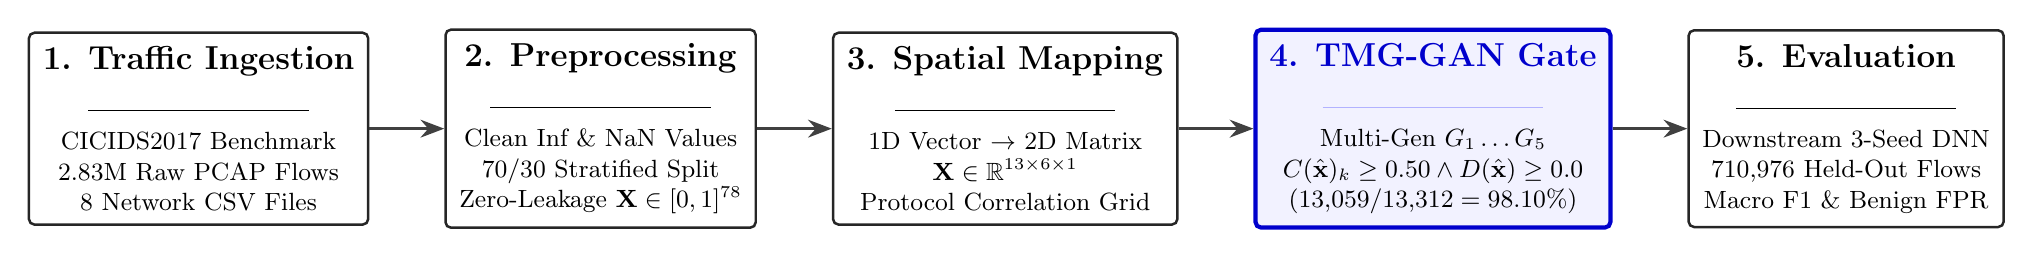
\begin{tikzpicture}[
    process/.style={
        draw=black!85,
        line width=0.9pt,
        rounded corners=2pt,
        minimum width=3.15cm,
        minimum height=1.65cm,
        align=center,
        font=\small,
        inner sep=5pt
    },
    gate/.style={
        draw=blue!80!black,
        line width=1.5pt,
        rounded corners=2pt,
        minimum width=3.15cm,
        minimum height=1.65cm,
        align=center,
        font=\small,
        inner sep=5pt,
        fill=blue!5
    },
    arrow/.style={
        -{Stealth[length=3mm]},
        line width=1.3pt,
        draw=black!75
    }
]
\node[process] (A) {
    \textbf{\large 1. Traffic Ingestion}\\[4pt]
    \rule{2.8cm}{0.4pt}\\[3pt]
    CICIDS2017 Benchmark\\
    2.83M Raw PCAP Flows\\
    8 Network CSV Files
};
\node[process, right=0.95cm of A] (B) {
    \textbf{\large 2. Preprocessing}\\[4pt]
    \rule{2.8cm}{0.4pt}\\[3pt]
    Clean Inf \& NaN Values\\
    70/30 Stratified Split\\
    Zero-Leakage $\mathbf{X}\in[0,1]^{78}$
};
\node[process, right=0.95cm of B] (C) {
    \textbf{\large 3. Spatial Mapping}\\[4pt]
    \rule{2.8cm}{0.4pt}\\[3pt]
    1D Vector $\rightarrow$ 2D Matrix\\
    $\mathbf{X}\in\mathbb{R}^{13\times6\times1}$\\
    Protocol Correlation Grid
};
\node[gate, right=0.95cm of C] (D) {
    \textcolor{blue!80!black}{\textbf{\large 4. TMG-GAN Gate}}\\[4pt]
    \textcolor{blue!30}{\rule{2.8cm}{0.4pt}}\\[3pt]
    Multi-Gen $G_1 \ldots G_5$\\
    $C(\hat{\mathbf{x}})_k \ge 0.50 \land D(\hat{\mathbf{x}}) \ge 0.0$\\
    ($13{,}059 / 13{,}312 = 98.10\%$)
};
\node[process, right=0.95cm of D] (E) {
    \textbf{\large 5. Evaluation}\\[4pt]
    \rule{2.8cm}{0.4pt}\\[3pt]
    Downstream 3-Seed DNN\\
    710,976 Held-Out Flows\\
    Macro F1 \& Benign FPR
};
\draw[arrow] (A.east) -- (B.west);
\draw[arrow] (B.east) -- (C.west);
\draw[arrow] (C.east) -- (D.west);
\draw[arrow] (D.east) -- (E.west);
\end{tikzpicture}%
}
\caption{End-to-end TMG-GAN pipeline illustrating traffic ingestion, preprocessing, spatial feature mapping, multi-generator sample quality filtering, and downstream evaluation.}
\label{fig:pipeline}
\end{figure*}

\section{Proposed Methodology}

The complete intrusion detection pipeline is illustrated in Fig.~\ref{fig:pipeline}. It consists of spatial flow representation, multi-generator modeling with spectral stabilization, and sample quality verification.

\subsection{Spatial Feature Representation}

Each network flow record comprises $D = 78$ continuous statistical attributes, such as forward inter-arrival time, flow duration, and packet length variance. Let $\mathbf{x} \in \mathbb{R}^{78}$ represent an individual flow vector, where $x_i$ denotes its $i$-th feature, and let $X_{i,\text{train}}$ be the set of $i$-th feature values across all training samples. Each feature is scaled to $[0, 1]$ using min-max normalization fitted strictly on training statistics:

\begin{equation}
\tilde{x}_i = \frac{x_i - \min(X_{i,\text{train}})}{\max(X_{i,\text{train}}) - \min(X_{i,\text{train}})}, \quad \forall i \in \{1, \dots, 78\}
\end{equation}

After normalization, the resulting 78-dimensional feature vector is reshaped into a two-dimensional matrix $\mathbf{X}_{\text{2D}} \in \mathbb{R}^{13 \times 6 \times 1}$. This spatial transformation enables $3 \times 3$ two-dimensional convolutional kernels to capture local structural patterns and cross-feature interactions among interrelated network statistics.

\subsection{TMG-GAN Multi-Generator Framework}

To avoid gradient interference across disparate attack types, an independent generator $G_k$ is assigned to each minority class $k \in \{1, \dots, 5\}$ (Denial-of-Service (DoS), PortScan, BruteForce, WebAttack, Bot). As shown in Fig.~\ref{fig:architecture}, each generator $G_k$ takes a latent noise vector $\mathbf{z} \sim \mathcal{N}(\mathbf{0}, \mathbf{I}_{128})$, where $\mathbf{0}$ is the zero vector and $\mathbf{I}_{128}$ is the $128 \times 128$ identity matrix, and projects it through multi-layer perceptrons with LeakyReLU activations into synthetic vectors:

\begin{equation}
\hat{\mathbf{x}}_k = G_k(\mathbf{z}; \theta_{G_k}) \in \mathbb{R}^{78}
\end{equation}
where $\hat{\mathbf{x}}_k$ denotes the generated feature vector and $\theta_{G_k}$ represents the trainable parameters of generator $G_k$.

\begin{figure*}[t]
\centering
\resizebox{\textwidth}{!}{%
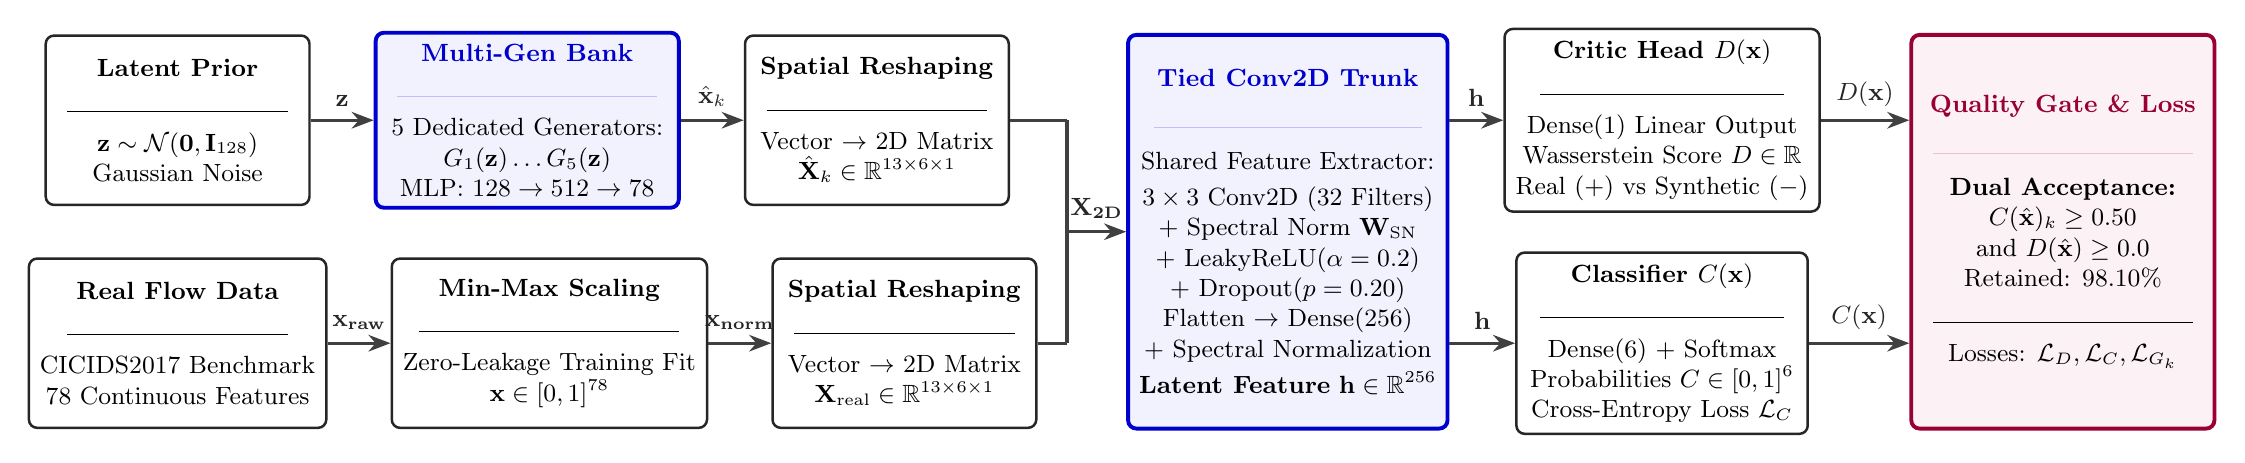
\begin{tikzpicture}[
    archbox/.style={
        draw=black!85,
        line width=0.9pt,
        rounded corners=3pt,
        minimum width=3.35cm,
        minimum height=2.15cm,
        align=center,
        font=\small,
        inner sep=4pt,
        fill=white
    },
    bluebox/.style={
        draw=blue!80!black,
        line width=1.4pt,
        rounded corners=3pt,
        minimum width=3.85cm,
        minimum height=2.15cm,
        align=center,
        font=\small,
        inner sep=4pt,
        fill=blue!5
    },
    trunkbox/.style={
        draw=blue!80!black,
        line width=1.4pt,
        rounded corners=3pt,
        minimum width=3.95cm,
        minimum height=5.0cm,
        align=center,
        font=\small,
        inner sep=4pt,
        fill=blue!5
    },
    gatebox/.style={
        draw=purple!80!black,
        line width=1.4pt,
        rounded corners=3pt,
        minimum width=3.85cm,
        minimum height=5.0cm,
        align=center,
        font=\small,
        inner sep=4pt,
        fill=purple!5
    },
    conn/.style={
        -{Stealth[length=2.8mm]},
        line width=1.2pt,
        draw=black!75
    },
    bus/.style={
        line width=1.2pt,
        draw=black!75
    },
    edgelabel/.style={
        font=\small\bfseries,
        text=black!85,
        above=1pt
    }
]
\node[archbox] (latent) {
    \textbf{Latent Prior}\\[2pt]
    \rule{2.8cm}{0.4pt}\\[3pt]
    $\mathbf{z} \sim \mathcal{N}(\mathbf{0}, \mathbf{I}_{128})$\\
    Gaussian Noise
};
\node[bluebox, right=0.8cm of latent] (multigen) {
    \textcolor{blue!80!black}{\textbf{Multi-Gen Bank}}\\[2pt]
    \textcolor{blue!25}{\rule{3.3cm}{0.4pt}}\\[3pt]
    5 Dedicated Generators:\\
    $G_1(\mathbf{z}) \dots G_5(\mathbf{z})$\\
    MLP: $128 \to 512 \to 78$
};
\node[archbox, right=0.8cm of multigen] (synmat) {
    \textbf{Spatial Reshaping}\\[2pt]
    \rule{2.8cm}{0.4pt}\\[3pt]
    Vector $\to$ 2D Matrix\\
    $\hat{\mathbf{X}}_k \in \mathbb{R}^{13 \times 6 \times 1}$
};
\node[archbox, below=0.65cm of latent] (realdata) {
    \textbf{Real Flow Data}\\[2pt]
    \rule{2.8cm}{0.4pt}\\[3pt]
    CICIDS2017 Benchmark\\
    78 Continuous Features
};
\node[archbox, right=0.8cm of realdata, minimum width=3.85cm] (norm) {
    \textbf{Min-Max Scaling}\\[2pt]
    \rule{3.3cm}{0.4pt}\\[3pt]
    Zero-Leakage Training Fit\\
    $\mathbf{x} \in [0, 1]^{78}$
};
\node[archbox, right=0.8cm of norm] (realmat) {
    \textbf{Spatial Reshaping}\\[2pt]
    \rule{2.8cm}{0.4pt}\\[3pt]
    Vector $\to$ 2D Matrix\\
    $\mathbf{X}_{\text{real}} \in \mathbb{R}^{13 \times 6 \times 1}$
};
\coordinate (midmat) at ($(synmat.east)!0.5!(realmat.east)$);
\node[trunkbox, right=1.3cm of midmat] (trunk) {
    \textcolor{blue!80!black}{\textbf{Tied Conv2D Trunk}}\\[4pt]
    \textcolor{blue!25}{\rule{3.4cm}{0.4pt}}\\[4pt]
    Shared Feature Extractor:\\[2pt]
    $3 \times 3$ Conv2D (32 Filters)\\
    $+$ Spectral Norm $\mathbf{W}_{\text{SN}}$\\
    $+$ LeakyReLU($\alpha = 0.2$)\\
    $+$ Dropout($p = 0.20$)\\
    Flatten $\to$ Dense(256)\\
    $+$ Spectral Normalization\\[2pt]
    \textbf{Latent Feature} $\mathbf{h} \in \mathbb{R}^{256}$
};
\node[archbox, minimum width=3.7cm] (critic) at ($(trunk.east |- synmat.center) + (2.7cm, 0)$) {
    \textbf{Critic Head $D(\mathbf{x})$}\\[2pt]
    \rule{3.1cm}{0.4pt}\\[3pt]
    Dense(1) Linear Output\\
    Wasserstein Score $D \in \mathbb{R}$\\
    Real ($+$) vs Synthetic ($-$)
};
\node[archbox, minimum width=3.7cm] (classifier) at ($(trunk.east |- realmat.center) + (2.7cm, 0)$) {
    \textbf{Classifier $C(\mathbf{x})$}\\[2pt]
    \rule{3.1cm}{0.4pt}\\[3pt]
    Dense(6) $+$ Softmax\\
    Probabilities $C \in [0, 1]^6$\\
    Cross-Entropy Loss $\mathcal{L}_C$
};
\coordinate (midheads) at ($(critic.east)!0.5!(classifier.east)$);
\node[gatebox, right=1.2cm of midheads] (gate) {
    \textcolor{purple!80!black}{\textbf{Quality Gate \& Loss}}\\[4pt]
    \textcolor{purple!25}{\rule{3.3cm}{0.4pt}}\\[4pt]
    \textbf{Dual Acceptance:}\\
    $C(\hat{\mathbf{x}})_k \ge 0.50$\\
    and $D(\hat{\mathbf{x}}) \ge 0.0$\\
    Retained: $98.10\%$\\[2pt]
    \rule{3.3cm}{0.2pt}\\[3pt]
    Losses: $\mathcal{L}_D, \mathcal{L}_C, \mathcal{L}_{G_k}$
};

\draw[conn] (latent.east) -- node[edgelabel] {$\mathbf{z}$} (multigen.west);
\draw[conn] (multigen.east) -- node[edgelabel] {$\hat{\mathbf{x}}_k$} (synmat.west);
\draw[conn] (realdata.east) -- node[edgelabel] {$\mathbf{x}_{\text{raw}}$} (norm.west);
\draw[conn] (norm.east) -- node[edgelabel] {$\mathbf{x}_{\text{norm}}$} (realmat.west);
\coordinate (busx) at ($(midmat) + (0.55cm, 0)$);
\draw[bus] (synmat.east) -- (synmat.east -| busx);
\draw[bus] (realmat.east) -- (realmat.east -| busx);
\draw[bus] (synmat.east -| busx) -- (realmat.east -| busx);
\draw[conn] (busx) -- node[edgelabel] {$\mathbf{X}_{\text{2D}}$} (trunk.west);
\draw[conn] (trunk.east |- critic.west) -- node[edgelabel] {$\mathbf{h}$} (critic.west);
\draw[conn] (trunk.east |- classifier.west) -- node[edgelabel] {$\mathbf{h}$} (classifier.west);
\draw[conn] (critic.east) -- node[edgelabel] {$D(\mathbf{x})$} (critic.east -| gate.west);
\draw[conn] (classifier.east) -- node[edgelabel] {$C(\mathbf{x})$} (classifier.east -| gate.west);
\end{tikzpicture}%
}
\caption{TMG-GAN neural architecture with a spectral-normalized two-dimensional convolutional (Conv2D) trunk, dual critic and auxiliary classifier heads, and a sample quality filtering gate.}
\label{fig:architecture}
\end{figure*}

The synthetic flows are reshaped to $13 \times 6 \times 1$ and fed to a shared convolutional discriminator/classifier network. The shared backbone contains a $3 \times 3$ two-dimensional convolutional (Conv2D) layer with 32 filters, LeakyReLU ($\alpha = 0.2$, where $\alpha$ is the negative-side slope) and Dropout ($p = 0.20$, where $p$ is the dropout probability), followed by a dense layer of 256 units. All weight matrices $\mathbf{W}$ are scaled by their spectral norm to improve training stability, following spectral normalization~\cite{miyato2018spectral}:

\begin{equation}
\mathbf{W}_{\text{SN}} = \frac{\mathbf{W}}{\sigma(\mathbf{W})}
\end{equation}
where $\mathbf{W}_{\text{SN}}$ is the normalized weight matrix, $\mathbf{W}$ is the original weight matrix, and $\sigma(\mathbf{W})$ is its largest singular value.

The shared representation branches into two output heads, defined as follows:

\begin{enumerate}
    \item \textbf{Realism Discriminator Head $D(\mathbf{x})$:} Computes a scalar Wasserstein realism score for an input flow. Its discriminator loss ($\mathcal{L}_D$) is calculated as the difference between the scores of real and generated flows, as expressed by
    \begin{equation}
    \mathcal{L}_D = \mathbb{E}_{\mathbf{x} \sim P_r}[D(\mathbf{x})] - \mathbb{E}_{\mathbf{z} \sim P_z}[D(G_k(\mathbf{z}))]
    \end{equation}
    where $P_r$ is the real-flow distribution, $P_z$ is the latent noise distribution, and $\mathbb{E}$ denotes mathematical expectation.

    \item \textbf{Auxiliary Classifier Head $C(\mathbf{x})$:} Computes class probabilities across all six classes using Softmax. Its classification loss ($\mathcal{L}_C$) is defined by the categorical cross-entropy between predicted probabilities and actual class labels, given by
    \begin{equation}
    \mathcal{L}_C = -\mathbb{E}_{(\mathbf{x}, y) \sim P_{\text{data}}} \left[ \sum_{c=0}^{5} y_c \log C(\mathbf{x})_c \right]
    \end{equation}
    where $P_{\text{data}}$ is the labeled training-data distribution, $y_c$ is the ground-truth indicator for class $c$, and $C(\mathbf{x})_c$ is the predicted probability of class $c$.
\end{enumerate}

To balance realism and target-class semantic fidelity, the generator loss ($\mathcal{L}_{G_k}$) is formulated by combining the adversarial, classification, and cosine similarity losses, as expressed by
\begin{equation}
\begin{aligned}
\mathcal{L}_{G_k} ={}&
-\mathbb{E}_{\mathbf{z} \sim P_z}[D(G_k(\mathbf{z}))]
\\
&+ \lambda_1 \mathcal{L}_C(G_k(\mathbf{z}), k)
\\
&+ \lambda_2 \mathcal{L}_{\text{cos}}(G_k(\mathbf{z}), \bar{\mathbf{x}}_k)
\end{aligned}
\end{equation}
where $\lambda_1$ and $\lambda_2$ are loss-weighting coefficients, $\mathcal{L}_{\text{cos}}$ measures cosine-based feature similarity, and $\bar{\mathbf{x}}_k$ is the empirical feature centroid of real training flows in minority class $k$.

\subsection{Sample Quality Filtering}

Generating synthetic samples near peripheral regions of the attack space may introduce label noise into downstream training. Therefore, each candidate flow $\hat{\mathbf{x}} = G_k(\mathbf{z})$ must pass two concurrent acceptance tests:

\begin{enumerate}
    \item \textbf{Classification Confidence Threshold:} The auxiliary classifier is required to assign a probability above the specified threshold to the intended target class $k$, satisfying
    \begin{equation}
    C(\hat{\mathbf{x}})_k \geq \tau_{\text{conf}} \quad (\tau_{\text{conf}} = 0.50)
    \end{equation}
    where $C(\hat{\mathbf{x}})_k$ is the predicted probability of class $k$ and $\tau_{\text{conf}}$ is the minimum confidence threshold.

    \item \textbf{Discriminator Realism Gate:} The discriminator output is required to exceed the specified threshold, satisfying
    \begin{equation}
    D(\hat{\mathbf{x}}) \geq \tau_D \quad (\tau_D = 0.0)
    \end{equation}
    where $D(\hat{\mathbf{x}})$ is the realism score and $\tau_D$ is the minimum acceptance threshold.
\end{enumerate}

A candidate is retained only when both conditions are satisfied. Experiments with this filter yield an empirical joint acceptance rate of $98.10\%$, retaining 13,059 high-quality synthetic flows for each of the five minority classes.

The overall training and augmentation procedure is summarized in Algorithm~\ref{alg:tmg_gan}. It combines class-specific generator training with confidence-based and discriminator-based filtering to construct the augmented training dataset.

\begin{algorithm}[t]
\caption{TMG-GAN Training and Augmentation}
\label{alg:tmg_gan}
\begin{algorithmic}[1]
\REQUIRE Real training set $\mathcal{D}_{\text{train}}$, batch size $m$, loss weights $\lambda_1, \lambda_2$, thresholds $\tau_{\text{conf}}, \tau_D$, target count $N$
\ENSURE Augmented training dataset $\mathcal{D}_{\text{aug}}$
\STATE Fit min-max scaler on $\mathcal{D}_{\text{train}}$ and reshape flows to $13 \times 6 \times 1$
\FOR{each training epoch}
    \FOR{each minority class $k \in \{1, \dots, 5\}$}
        \STATE Sample minibatch of real flows $\mathbf{x} \sim P_{r,k}$
        \STATE Sample noise $\mathbf{z} \sim \mathcal{N}(\mathbf{0}, \mathbf{I}_{128})$, generate $\hat{\mathbf{x}}_k = G_k(\mathbf{z})$
        \STATE Update shared trunk and heads via $\mathcal{L}_D$ and $\mathcal{L}_C$
        \STATE Update generator $G_k$ via $\mathcal{L}_{G_k}$ with spectral normalization
    \ENDFOR
\ENDFOR
\STATE Initialize $\mathcal{D}_{\text{aug}} \leftarrow \mathcal{D}_{\text{train}}$
\FOR{each minority class $k \in \{1, \dots, 5\}$}
    \STATE Initialize accepted set $\mathcal{S}_k \leftarrow \emptyset$
    \WHILE{$|\mathcal{S}_k| < N$}
        \STATE Sample noise $\mathbf{z} \sim \mathcal{N}(\mathbf{0}, \mathbf{I}_{128})$ and generate candidate $\hat{\mathbf{x}} = G_k(\mathbf{z})$
        \IF{$C(\hat{\mathbf{x}})_k \geq \tau_{\text{conf}}$ \AND $D(\hat{\mathbf{x}}) \geq \tau_D$}
            \STATE $\mathcal{S}_k \leftarrow \mathcal{S}_k \cup \{(\hat{\mathbf{x}}, k)\}$
        \ENDIF
    \ENDWHILE
    \STATE $\mathcal{D}_{\text{aug}} \leftarrow \mathcal{D}_{\text{aug}} \cup \mathcal{S}_k$
\ENDFOR
\RETURN $\mathcal{D}_{\text{aug}}$
\end{algorithmic}
\end{algorithm}


\section{Performance Evaluation and Analysis}

\subsection{Dataset and Experimental Setup}

The approach is validated on the Canadian Institute for Cybersecurity CICIDS2017 dataset~\cite{sharafaldin2018toward}, which contains 2,830,743 raw network flows across eight CSV files captured over a 5-day monitoring period.

To prevent methodological bias and information leakage, the following preprocessing protocol is applied:
\begin{itemize}\setlength{\itemsep}{2pt}\setlength{\topsep}{2pt}\setlength{\parsep}{0pt}
    \item \textbf{Cleaning:} Rows containing infinite or missing values are dropped, leaving 2,827,876 valid flows. After removing duplicate flow records, 2,520,798 clean flows remain.
    \item \textbf{Class Aggregation:} Attack types are mapped into six canonical classes: Benign, DoS, PortScan, BruteForce, WebAttack, and Bot.
    \item \textbf{Stratified Partitioning:} The data are partitioned using a stratified 70\%/30\% split. Following the experimental design of Ding et al.~\cite{ding2024tmggan}, the training pool is subsampled to construct an imbalanced training set of 145,149 flows, while the held-out test partition is evaluated in its entirety (710,976 flows, containing 621,677 Benign flows) to assess performance under realistic network operational distributions.
    \item \textbf{Strict Zero-Leakage Normalization:} The min-max scaler is fitted strictly on the 145,149 training flows and serialized; the held-out test set is transformed purely using these training statistics without information leakage.
\end{itemize}

As shown in Table~\ref{tab:dataset_distribution}, benign traffic comprises 105,222 flows (72.49\%) of the training partition, while DoS accounts for 27,816 flows (19.16\%) and PortScan accounts for 9,735 flows (6.71\%). The remaining three attack categories are severely underrepresented: BruteForce comprises 943 flows (0.65\%), WebAttack comprises 576 flows (0.40\%), and Bot comprises 857 flows (0.59\%).

\begin{table}[t]
\centering
\caption{Class Distribution in Preprocessed CICIDS2017 Dataset}
\label{tab:dataset_distribution}
\begin{tabular}{lrrrr}
\toprule
\textbf{Class} & \textbf{Train Flows} & \textbf{Ratio (\%)} & \textbf{Test Flows} & \textbf{Ratio (\%)} \\
\midrule
Benign      & 105,222 & 72.49\% & 621,677 & 87.44\% \\
DoS         &  27,816 & 19.16\% &  64,904 &  9.13\% \\
PortScan    &   9,735 &  6.71\% &  22,714 &  3.19\% \\
BruteForce  &     943 &  0.65\% &     460 &  0.06\% \\
WebAttack   &     576 &  0.40\% &     114 &  0.02\% \\
Bot         &     857 &  0.59\% &   1,107 &  0.16\% \\
\midrule
\textbf{Total} & \textbf{145,149} & \textbf{100.00\%} & \textbf{710,976} & \textbf{100.00\%} \\
\bottomrule
\end{tabular}
\end{table}

The experiments are conducted on a computer system equipped with a 12th Generation Intel Core i7 processor, 16~GB of RAM, and an NVIDIA GeForce RTX 3050 graphics processing unit (GPU) with 4~GB of dedicated graphics memory. The central processing unit (CPU) is used for data preprocessing, feature extraction, and general computational tasks, while the graphics processing unit (GPU) accelerates the training process of the GAN architecture. All experiments are implemented using PyTorch with CUDA acceleration.

For a strictly controlled comparison, all evaluated training configurations (DNN without augmentation, DNN + SMOTE, DNN + ADASYN, and DNN + TMG-GAN) use an identical Deep Neural Network (DNN) downstream classifier. The downstream classifier contains three fully connected layers with dimensions $78 \to 256 \to 128 \to 6$. It uses LeakyReLU activations ($\alpha = 0.2$), batch normalization, and dropout ($p = 0.20$).

Each model is trained for 50 epochs using the Adam optimizer with an initial learning rate of $1 \times 10^{-3}$, cosine annealing schedule, and batch size of 256. All experiments are conducted across three independent random seeds ($0, 1, 2$), ensuring that the reported results reflect statistical repeatability.

\subsection{Results}

\subsubsection{Primary Evaluation: Macro Performance and False-Alarm Dynamics}

The aggregate classification results for the evaluated training configurations are summarized in Table~\ref{tab:evaluation_results}.

\begin{table*}[t]
\centering
\caption{Aggregate Performance on Held-Out CICIDS2017 Test Set (Mean $\pm$ Std across 3 Seeds)}
\label{tab:evaluation_results}
\resizebox{\textwidth}{!}{%
\begin{tabular}{lccccc}
\toprule
\textbf{Configuration} & \textbf{Train Size} & \textbf{Macro Prec. (\%)} & \textbf{Macro Rec. (\%)} & \textbf{Macro F1} & \textbf{Benign FPR (\%)} \\
\midrule
DNN (Original)                 & 145,149 & $71.25 \pm 2.01$ & $96.71 \pm 1.81$ & $0.7813 \pm 0.0117$ & $2.4716 \pm 0.0664$ \\
DNN + SMOTE                    & 210,444 & $68.29 \pm 0.77$ & $99.19 \pm 0.02$ & $0.7518 \pm 0.0102$ & $2.6366 \pm 0.0798$ \\
DNN + ADASYN                   & 210,880 & $67.11 \pm 1.25$ & $\mathbf{99.36 \pm 0.03}$ & $0.7390 \pm 0.0148$ & $2.9324 \pm 0.1141$ \\
\textbf{DNN + TMG-GAN (Prop.)} & 210,444 & $\mathbf{73.41 \pm 3.28}$ & $95.23 \pm 2.57$ & $\mathbf{0.7940 \pm 0.0237}$ & $\mathbf{2.3088 \pm 0.2161}$ \\
\bottomrule
\end{tabular}%
}
\end{table*}

Table~\ref{tab:evaluation_results} reports aggregate metrics across the 710,976 held-out test flows. DNN (Without Augmentation) achieves a macro F1-score of $0.7813 \pm 0.0117$. While DNN + SMOTE improves macro recall to $99.19\% \pm 0.02\%$ and DNN + ADASYN achieves $99.36\% \pm 0.03\%$, both interpolation techniques significantly degrade macro precision ($68.29\%$ and $67.11\%$, respectively) and reduce the overall macro F1-score ($0.7518$ and $0.7390$).

In contrast, \textbf{DNN + TMG-GAN (Proposed)} achieves the highest macro F1-score of $\mathbf{0.7940 \pm 0.0237}$ and highest macro precision of $\mathbf{73.41\% \pm 3.28\%}$.

The benign false-positive rates of the evaluated training configurations are compared in Fig.~\ref{fig:benign_fpr}.

\begin{figure}[t]
\centering
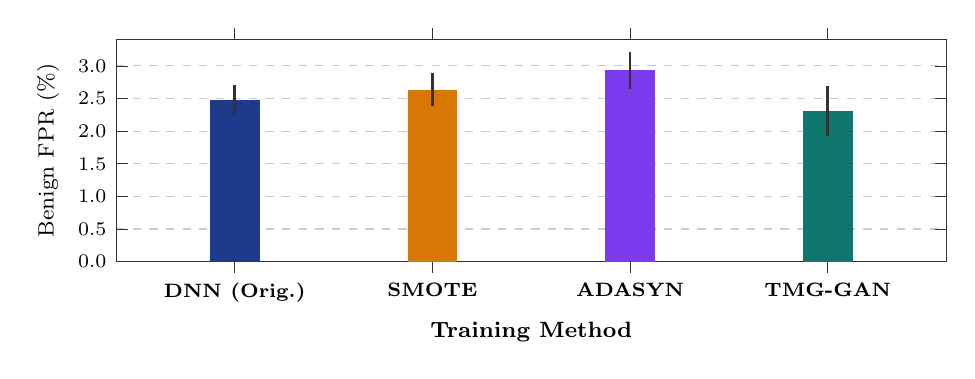
\begin{tikzpicture}
\begin{axis}[
    ybar,
    bar width=18pt,
    bar shift=0pt,
    width=\columnwidth,
    height=4.4cm,
    ymin=0,
    ymax=3.4,
    ytick={0.0, 0.5, 1.0, 1.5, 2.0, 2.5, 3.0},
    yticklabels={0.0, 0.5, 1.0, 1.5, 2.0, 2.5, 3.0},
    ymajorgrids=true,
    grid style={dashed, gray!40},
    axis on top=false,
    enlarge x limits=0.20,
    xtick={0, 1, 2, 3},
    xticklabels={DNN (Orig.), SMOTE, ADASYN, TMG-GAN},
    xticklabel style={font=\scriptsize\bfseries},
    yticklabel style={font=\scriptsize},
    xlabel={Training Method},
    xlabel style={font=\footnotesize\bfseries},
    ylabel={Benign FPR (\%)},
    ylabel style={font=\footnotesize},
    axis line style={black!80},
    tick style={black!80}
]
\addplot[
    fill=origblue,
    draw=none,
    error bars/.cd,
    y dir=both,
    y explicit,
    error mark=-,
    error bar style={line width=1.0pt, color=black!80},
    error mark options={mark size=4pt, line width=1.0pt, color=black!80}
] coordinates {(0, 2.4716) +- (0, 0.0664)};
\addplot[
    fill=smoteorange,
    draw=none,
    error bars/.cd,
    y dir=both,
    y explicit,
    error mark=-,
    error bar style={line width=1.0pt, color=black!80},
    error mark options={mark size=4pt, line width=1.0pt, color=black!80}
] coordinates {(1, 2.6366) +- (0, 0.0798)};
\addplot[
    fill=adasynpurple,
    draw=none,
    error bars/.cd,
    y dir=both,
    y explicit,
    error mark=-,
    error bar style={line width=1.0pt, color=black!80},
    error mark options={mark size=4pt, line width=1.0pt, color=black!80}
] coordinates {(2, 2.9324) +- (0, 0.1141)};
\addplot[
    fill=tmggreen,
    draw=none,
    error bars/.cd,
    y dir=both,
    y explicit,
    error mark=-,
    error bar style={line width=1.0pt, color=black!80},
    error mark options={mark size=4pt, line width=1.0pt, color=black!80}
] coordinates {(3, 2.3088) +- (0, 0.2161)};
\end{axis}
\end{tikzpicture}
\caption{Benign false-positive rate (FPR) across baseline and augmented configurations on $621{,}677$ normal test flows (mean $\pm$ standard deviation across three random seeds).}
\label{fig:benign_fpr}
\end{figure}

As illustrated in Fig.~\ref{fig:benign_fpr}, the operational impact on the benign false-positive rate is substantial:
\begin{itemize}\setlength{\itemsep}{2pt}\setlength{\topsep}{2pt}\setlength{\parsep}{0pt}
    \item \textbf{SMOTE and ADASYN Boundary Inflation:} DNN + SMOTE increases benign FPR from $2.4716\%$ to $2.6366\%$ (an additional 1,026 false alarms on 621,677 benign flows), while DNN + ADASYN elevates benign FPR to $2.9324\%$ (an extra 2,865 false alarms).
    \item \textbf{TMG-GAN Suppression:} DNN + TMG-GAN (Proposed) reduces benign FPR to $\mathbf{2.3088\% \pm 0.2161\%}$, producing 14,353 false alarms. This represents 2,038 fewer false alarms than SMOTE and 3,877 fewer false alarms than ADASYN, substantially mitigating alert fatigue.
\end{itemize}

\subsubsection{Sample Quality Filtering Ablation Study}

To rigorously evaluate the contribution of the sample quality filtering mechanism, an ablation study was conducted comparing three generation arms under identical experimental conditions and random seeds ($0, 1, 2$):
\begin{itemize}\setlength{\itemsep}{2pt}\setlength{\topsep}{2pt}\setlength{\parsep}{0pt}
    \item \textbf{Arm A (Unfiltered Generator):} Raw generator candidates without post-generation quality filtering.
    \item \textbf{Arm B (Classifier Gate Only):} Retains candidates that satisfy the auxiliary classifier argmax agreement criterion $\arg\max_j C(\hat{\mathbf{x}})_j = k$.
    \item \textbf{Arm C (Dual-Criterion Gate):} Retains candidates that satisfy both classifier confidence ($C(\hat{\mathbf{x}})_k \geq 0.50$) and discriminator realism ($D(\hat{\mathbf{x}}) \geq 0.0$).
\end{itemize}

The ablation results on the 710,976 held-out test flows are presented in Table~\ref{tab:ablation}.

\begin{table*}[t]
\centering
\caption{Ablation Study of Sample Quality Filtering on Held-Out Test Set (Mean $\pm$ Std across 3 Seeds)}
\label{tab:ablation}
\resizebox{\textwidth}{!}{%
\begin{tabular}{lcccccc}
\toprule
\textbf{Ablation Arm} & \textbf{Filter Criterion} & \textbf{Accept. (\%)} & \textbf{Macro Prec. (\%)} & \textbf{Macro Rec. (\%)} & \textbf{Macro F1} & \textbf{Benign FPR (\%)} \\
\midrule
Arm A (None)       & Unfiltered ($G_k$ raw) & 100.00\% & $73.70 \pm 3.53$ & $95.75 \pm 2.20$ & $0.7975 \pm 0.0278$ & $2.3000 \pm 0.2054$ \\
Arm B (Classifier) & $C(\hat{\mathbf{x}})_k \ge 0.50$ &  98.10\% & $73.81 \pm 3.75$ & $95.58 \pm 2.34$ & $0.7978 \pm 0.0287$ & $2.3058 \pm 0.2168$ \\
Arm C (Dual Gate)  & $C_k \ge 0.50 \land D \ge 0.0$ &  98.10\% & $73.41 \pm 3.28$ & $95.23 \pm 2.57$ & $0.7940 \pm 0.0237$ & $2.3088 \pm 0.2161$ \\
\bottomrule
\end{tabular}%
}
\end{table*}

The ablation analysis reveals that all three TMG-GAN variants achieve comparable downstream macro F1-scores ($0.7940$--$0.7978$) and benign false-positive rates ($\approx 2.30\%$--$2.31\%$), decisively outperforming the SMOTE ($0.7518$) and ADASYN ($0.7390$) baselines. The dual-criterion gate in Arm C filters out approximately $1.90\%$ of borderline candidate flows, functioning effectively as an automated quality assurance filter without compromising downstream attack recall.

\subsubsection{Per-Class Granular Breakdown}

The detailed precision, recall, and F1-score values for each traffic class are reported in Table~\ref{tab:per_class_results}.

\begin{table}[t]
\centering
\caption{Per-Class Classification Metrics on 710,976 Held-Out Test Flows (Mean across 3 Seeds)}
\label{tab:per_class_results}
\footnotesize
\setlength{\tabcolsep}{3.8pt}
\begin{tabular}{llcccc}
\toprule
\textbf{Class} & \textbf{Metric} & \textbf{Original} & \textbf{SMOTE} & \textbf{ADASYN} & \textbf{TMG-GAN} \\
\midrule
\multirow{3}{*}{Benign}     & Precision (\%) & 99.97 & 99.99 & 99.99 & 99.96 \\
                            & Recall (\%)    & 97.53 & 97.36 & 97.07 & \textbf{97.69} \\
                            & F1-Score       & 0.9874 & 0.9866 & 0.9851 & \textbf{0.9881} \\
\midrule
\multirow{3}{*}{DoS}        & Precision (\%) & 95.38 & 95.98 & 94.98 & \textbf{96.19} \\
                            & Recall (\%)    & 99.93 & 99.90 & 99.90 & 99.86 \\
                            & F1-Score       & 0.9760 & 0.9790 & 0.9738 & \textbf{0.9799} \\
\midrule
\multirow{3}{*}{PortScan}   & Precision (\%) & 74.33 & 74.26 & 74.24 & 74.25 \\
                            & Recall (\%)    & 99.76 & 99.90 & 99.91 & 99.86 \\
                            & F1-Score       & 0.8519 & 0.8519 & 0.8518 & 0.8517 \\
\midrule
\multirow{3}{*}{BruteForce} & Precision (\%) & 93.21 & 95.45 & 92.80 & \textbf{96.24} \\
                            & Recall (\%)    & 99.72 & 99.76 & \textbf{100.00} & 99.54 \\
                            & F1-Score       & 0.9635 & 0.9755 & 0.9627 & \textbf{0.9785} \\
\midrule
\multirow{3}{*}{WebAttack}  & Precision (\%) & 21.68 & 20.24 & 27.26 & \textbf{25.53} \\
                            & Recall (\%)    & 96.47 & 99.64 & \textbf{99.95} & 97.46 \\
                            & F1-Score       & 0.3541 & 0.3364 & 0.4248 & \textbf{0.4016} \\
\midrule
\multirow{3}{*}{Bot}        & Precision (\%) & 42.91 & 23.81 & 13.39 & \textbf{48.27} \\
                            & Recall (\%)    & 86.87 & 98.57 & \textbf{99.32} & 76.99 \\
                            & F1-Score       & 0.5548 & 0.3811 & 0.2359 & \textbf{0.5641} \\
\bottomrule
\end{tabular}
\end{table}

The per-class recall values are compared in Fig.~\ref{fig:recall_by_class}.

\begin{figure}[t]
\centering
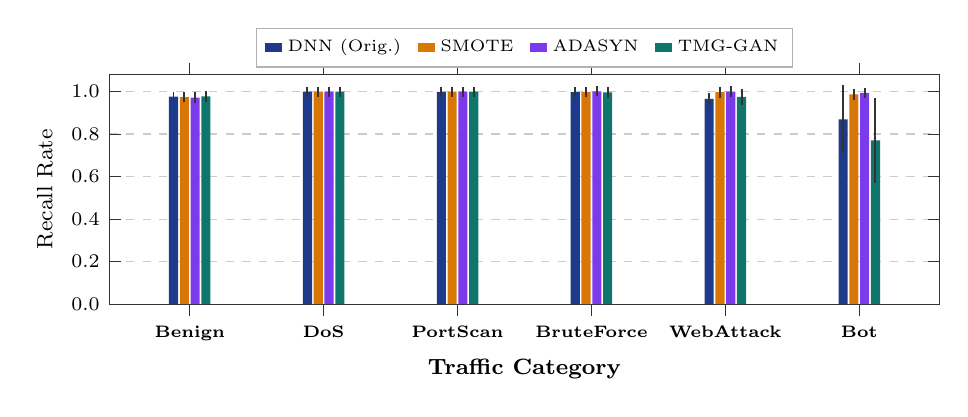
\begin{tikzpicture}
\begin{axis}[
    ybar=0.6pt,
    bar width=3.3pt,
    width=\columnwidth,
    height=4.5cm,
    ymin=0.0,
    ymax=1.08,
    ytick={0.0, 0.2, 0.4, 0.6, 0.8, 1.0},
    yticklabels={0.0, 0.2, 0.4, 0.6, 0.8, 1.0},
    ymajorgrids=true,
    grid style={dashed, gray!40},
    axis on top=false,
    symbolic x coords={Benign, DoS, PortScan, BruteForce, WebAttack, Bot},
    xtick=data,
    enlarge x limits=0.12,
    xticklabel style={font=\fontsize{6.2}{7.2}\selectfont\bfseries},
    yticklabel style={font=\scriptsize},
    xlabel={Traffic Category},
    xlabel style={font=\footnotesize\bfseries},
    ylabel={Recall Rate},
    ylabel style={font=\footnotesize},
    legend style={
        at={(0.5, 1.03)},
        anchor=south,
        legend columns=4,
        font=\fontsize{5.8}{6.8}\selectfont,
        fill=white,
        draw=black!30,
        /tikz/every even column/.append style={column sep=4pt}
    },
    legend image code/.code={%
        \draw[#1, draw=none] (0cm,-0.06cm) rectangle (0.22cm,0.06cm);
    },
    axis line style={black!80},
    tick style={black!80}
]
\addplot[
    fill=origblue,
    draw=none,
    error bars/.cd,
    y dir=both,
    y explicit,
    error mark=-,
    error bar style={line width=0.7pt, color=black!80},
    error mark options={mark size=1.8pt, line width=0.7pt, color=black!80}
] coordinates {
    (Benign, 0.9753) +- (0, 0.0008)
    (DoS, 0.9993) +- (0, 0.0002)
    (PortScan, 0.9976) +- (0, 0.0011)
    (BruteForce, 0.9972) +- (0, 0.0002)
    (WebAttack, 0.9647) +- (0, 0.0045)
    (Bot, 0.8687) +- (0, 0.1359)
};
\addlegendentry{DNN (Orig.)}

\addplot[
    fill=smoteorange,
    draw=none,
    error bars/.cd,
    y dir=both,
    y explicit,
    error mark=-,
    error bar style={line width=0.7pt, color=black!80},
    error mark options={mark size=1.8pt, line width=0.7pt, color=black!80}
] coordinates {
    (Benign, 0.9736) +- (0, 0.0010)
    (DoS, 0.9990) +- (0, 0.0002)
    (PortScan, 0.9990) +- (0, 0.0001)
    (BruteForce, 0.9976) +- (0, 0.0009)
    (WebAttack, 0.9964) +- (0, 0.0024)
    (Bot, 0.9857) +- (0, 0.0026)
};
\addlegendentry{SMOTE}

\addplot[
    fill=adasynpurple,
    draw=none,
    error bars/.cd,
    y dir=both,
    y explicit,
    error mark=-,
    error bar style={line width=0.7pt, color=black!80},
    error mark options={mark size=1.8pt, line width=0.7pt, color=black!80}
] coordinates {
    (Benign, 0.9707) +- (0, 0.0012)
    (DoS, 0.9990) +- (0, 0.0003)
    (PortScan, 0.9991) +- (0, 0.0001)
    (BruteForce, 1.0000) +- (0, 0.0000)
    (WebAttack, 0.9995) +- (0, 0.0008)
    (Bot, 0.9932) +- (0, 0.0017)
};
\addlegendentry{ADASYN}

\addplot[
    fill=tmggreen,
    draw=none,
    error bars/.cd,
    y dir=both,
    y explicit,
    error mark=-,
    error bar style={line width=0.7pt, color=black!80},
    error mark options={mark size=1.8pt, line width=0.7pt, color=black!80}
] coordinates {
    (Benign, 0.9769) +- (0, 0.0026)
    (DoS, 0.9986) +- (0, 0.0006)
    (PortScan, 0.9986) +- (0, 0.0003)
    (BruteForce, 0.9954) +- (0, 0.0012)
    (WebAttack, 0.9746) +- (0, 0.0134)
    (Bot, 0.7700) +- (0, 0.1770)
};
\addlegendentry{TMG-GAN}
\end{axis}
\end{tikzpicture}
\caption{Per-class recall comparison across the four evaluated DNN training configurations on $710{,}976$ held-out test flows.}
\label{fig:recall_by_class}
\end{figure}

Table~\ref{tab:per_class_results} presents detailed per-class results across all six categories:
\begin{itemize}\setlength{\itemsep}{2pt}\setlength{\topsep}{2pt}\setlength{\parsep}{0pt}
    \item \textbf{Botnet Detection:} For the rarest class (Bot, 857 training flows), DNN + SMOTE achieves $98.57\%$ recall and ADASYN achieves $99.32\%$ recall, but their precisions drop severely to $23.81\%$ and $13.39\%$, respectively. DNN + TMG-GAN (Proposed) maintains a much higher precision of $\mathbf{48.27\%}$ while achieving the highest F1-score of $\mathbf{0.5641}$.
    \item \textbf{Web Attacks:} On WebAttack, DNN + TMG-GAN (Proposed) improves precision over SMOTE ($25.53\%$ versus $20.24\%$) and achieves an F1-score of $0.4016$ versus $0.3364$ for SMOTE.
    \item \textbf{Benign Stability:} On benign flows, DNN + TMG-GAN (Proposed) records the highest recall ($97.69\%$), preventing false misclassifications on normal network traffic.
\end{itemize}

\subsubsection{Confusion Matrix and Latent Space Analysis}

The normalized confusion matrix for the proposed downstream classifier is shown in Fig.~\ref{fig:confusion}.

\begin{figure}[t]
\centering
\resizebox{0.94\columnwidth}{!}{%
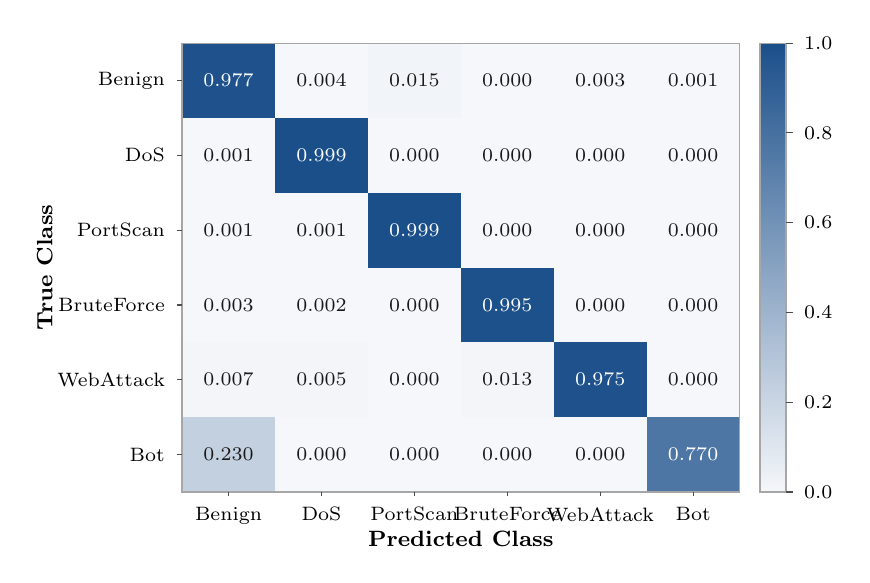
\begin{tikzpicture}[x=1.18cm, y=0.95cm, font=\scriptsize]
\foreach \r/\c/\val/\pct/\dark in {
    0/0/0.977/98/1, 0/1/0.004/0/0, 0/2/0.015/2/0, 0/3/0.000/0/0, 0/4/0.003/0/0, 0/5/0.001/0/0,
    1/0/0.001/0/0, 1/1/0.999/100/1, 1/2/0.000/0/0, 1/3/0.000/0/0, 1/4/0.000/0/0, 1/5/0.000/0/0,
    2/0/0.001/0/0, 2/1/0.001/0/0, 2/2/0.999/100/1, 2/3/0.000/0/0, 2/4/0.000/0/0, 2/5/0.000/0/0,
    3/0/0.003/0/0, 3/1/0.002/0/0, 3/2/0.000/0/0, 3/3/0.995/99/1, 3/4/0.000/0/0, 3/5/0.000/0/0,
    4/0/0.007/1/0, 4/1/0.005/1/0, 4/2/0.000/0/0, 4/3/0.013/1/0, 4/4/0.975/98/1, 4/5/0.000/0/0,
    5/0/0.230/23/0, 5/1/0.000/0/0, 5/2/0.000/0/0, 5/3/0.000/0/0, 5/4/0.000/0/0, 5/5/0.770/77/1
}{
    \fill[cmblue!\pct!cmwhite] (\c, -\r) rectangle (\c+1, -\r-1);
    \ifnum\dark=1
        \node[text=white] at (\c+0.5, -\r-0.5) {\val};
    \else
        \node[text=black!90] at (\c+0.5, -\r-0.5) {\val};
    \fi
}
\draw[black!35, line width=0.45pt] (0,0) rectangle (6,-6);
\foreach \r/\lbl in {0/Benign, 1/DoS, 2/PortScan, 3/BruteForce, 4/WebAttack, 5/Bot} {
    \node[anchor=east, font=\scriptsize] at (-0.08, -\r-0.5) {\lbl};
    \draw[black!70] (0, -\r-0.5) -- (-0.06, -\r-0.5);
}
\node[rotate=90, font=\footnotesize\bfseries] at (-1.48, -3.0) {True Class};
\foreach \c/\lbl in {0/Benign, 1/DoS, 2/PortScan, 3/BruteForce, 4/WebAttack, 5/Bot} {
    \node[anchor=north, font=\scriptsize] at (\c+0.5, -6.08) {\lbl};
    \draw[black!70] (\c+0.5, -6.0) -- (\c+0.5, -6.06);
}
\node[font=\footnotesize\bfseries] at (3.0, -6.62) {Predicted Class};
\shade[top color=cmblue, bottom color=cmwhite] (6.22, -6.0) rectangle (6.50, 0.0);
\draw[black!35, line width=0.4pt] (6.22, -6.0) rectangle (6.50, 0.0);
\foreach \ypos/\lbl in {-6.0/0.0, -4.8/0.2, -3.6/0.4, -2.4/0.6, -1.2/0.8, 0.0/1.0} {
    \draw[black!70] (6.50, \ypos) -- (6.57, \ypos);
    \node[anchor=west, font=\scriptsize] at (6.59, \ypos) {\lbl};
}
\end{tikzpicture}%
}
\caption{Normalized confusion matrix of the DNN + TMG-GAN (Proposed) downstream classifier on $710{,}976$ held-out test flows.}
\label{fig:confusion}
\end{figure}

Fig.~\ref{fig:confusion} displays the normalized confusion matrix for DNN + TMG-GAN (Proposed), showing diagonal accuracies of $97.7\%$ on Benign flows, $99.9\%$ on DoS, $99.9\%$ on PortScan, $99.5\%$ on BruteForce, $97.5\%$ on WebAttack, and $77.0\%$ on Bot flows. Crucially, benign misclassification is suppressed, maintaining stable classification boundaries.

The distribution of real and synthetic attack flows in the latent feature space is visualized in Fig.~\ref{fig:tsne}.

\begin{figure}[t]
\centering
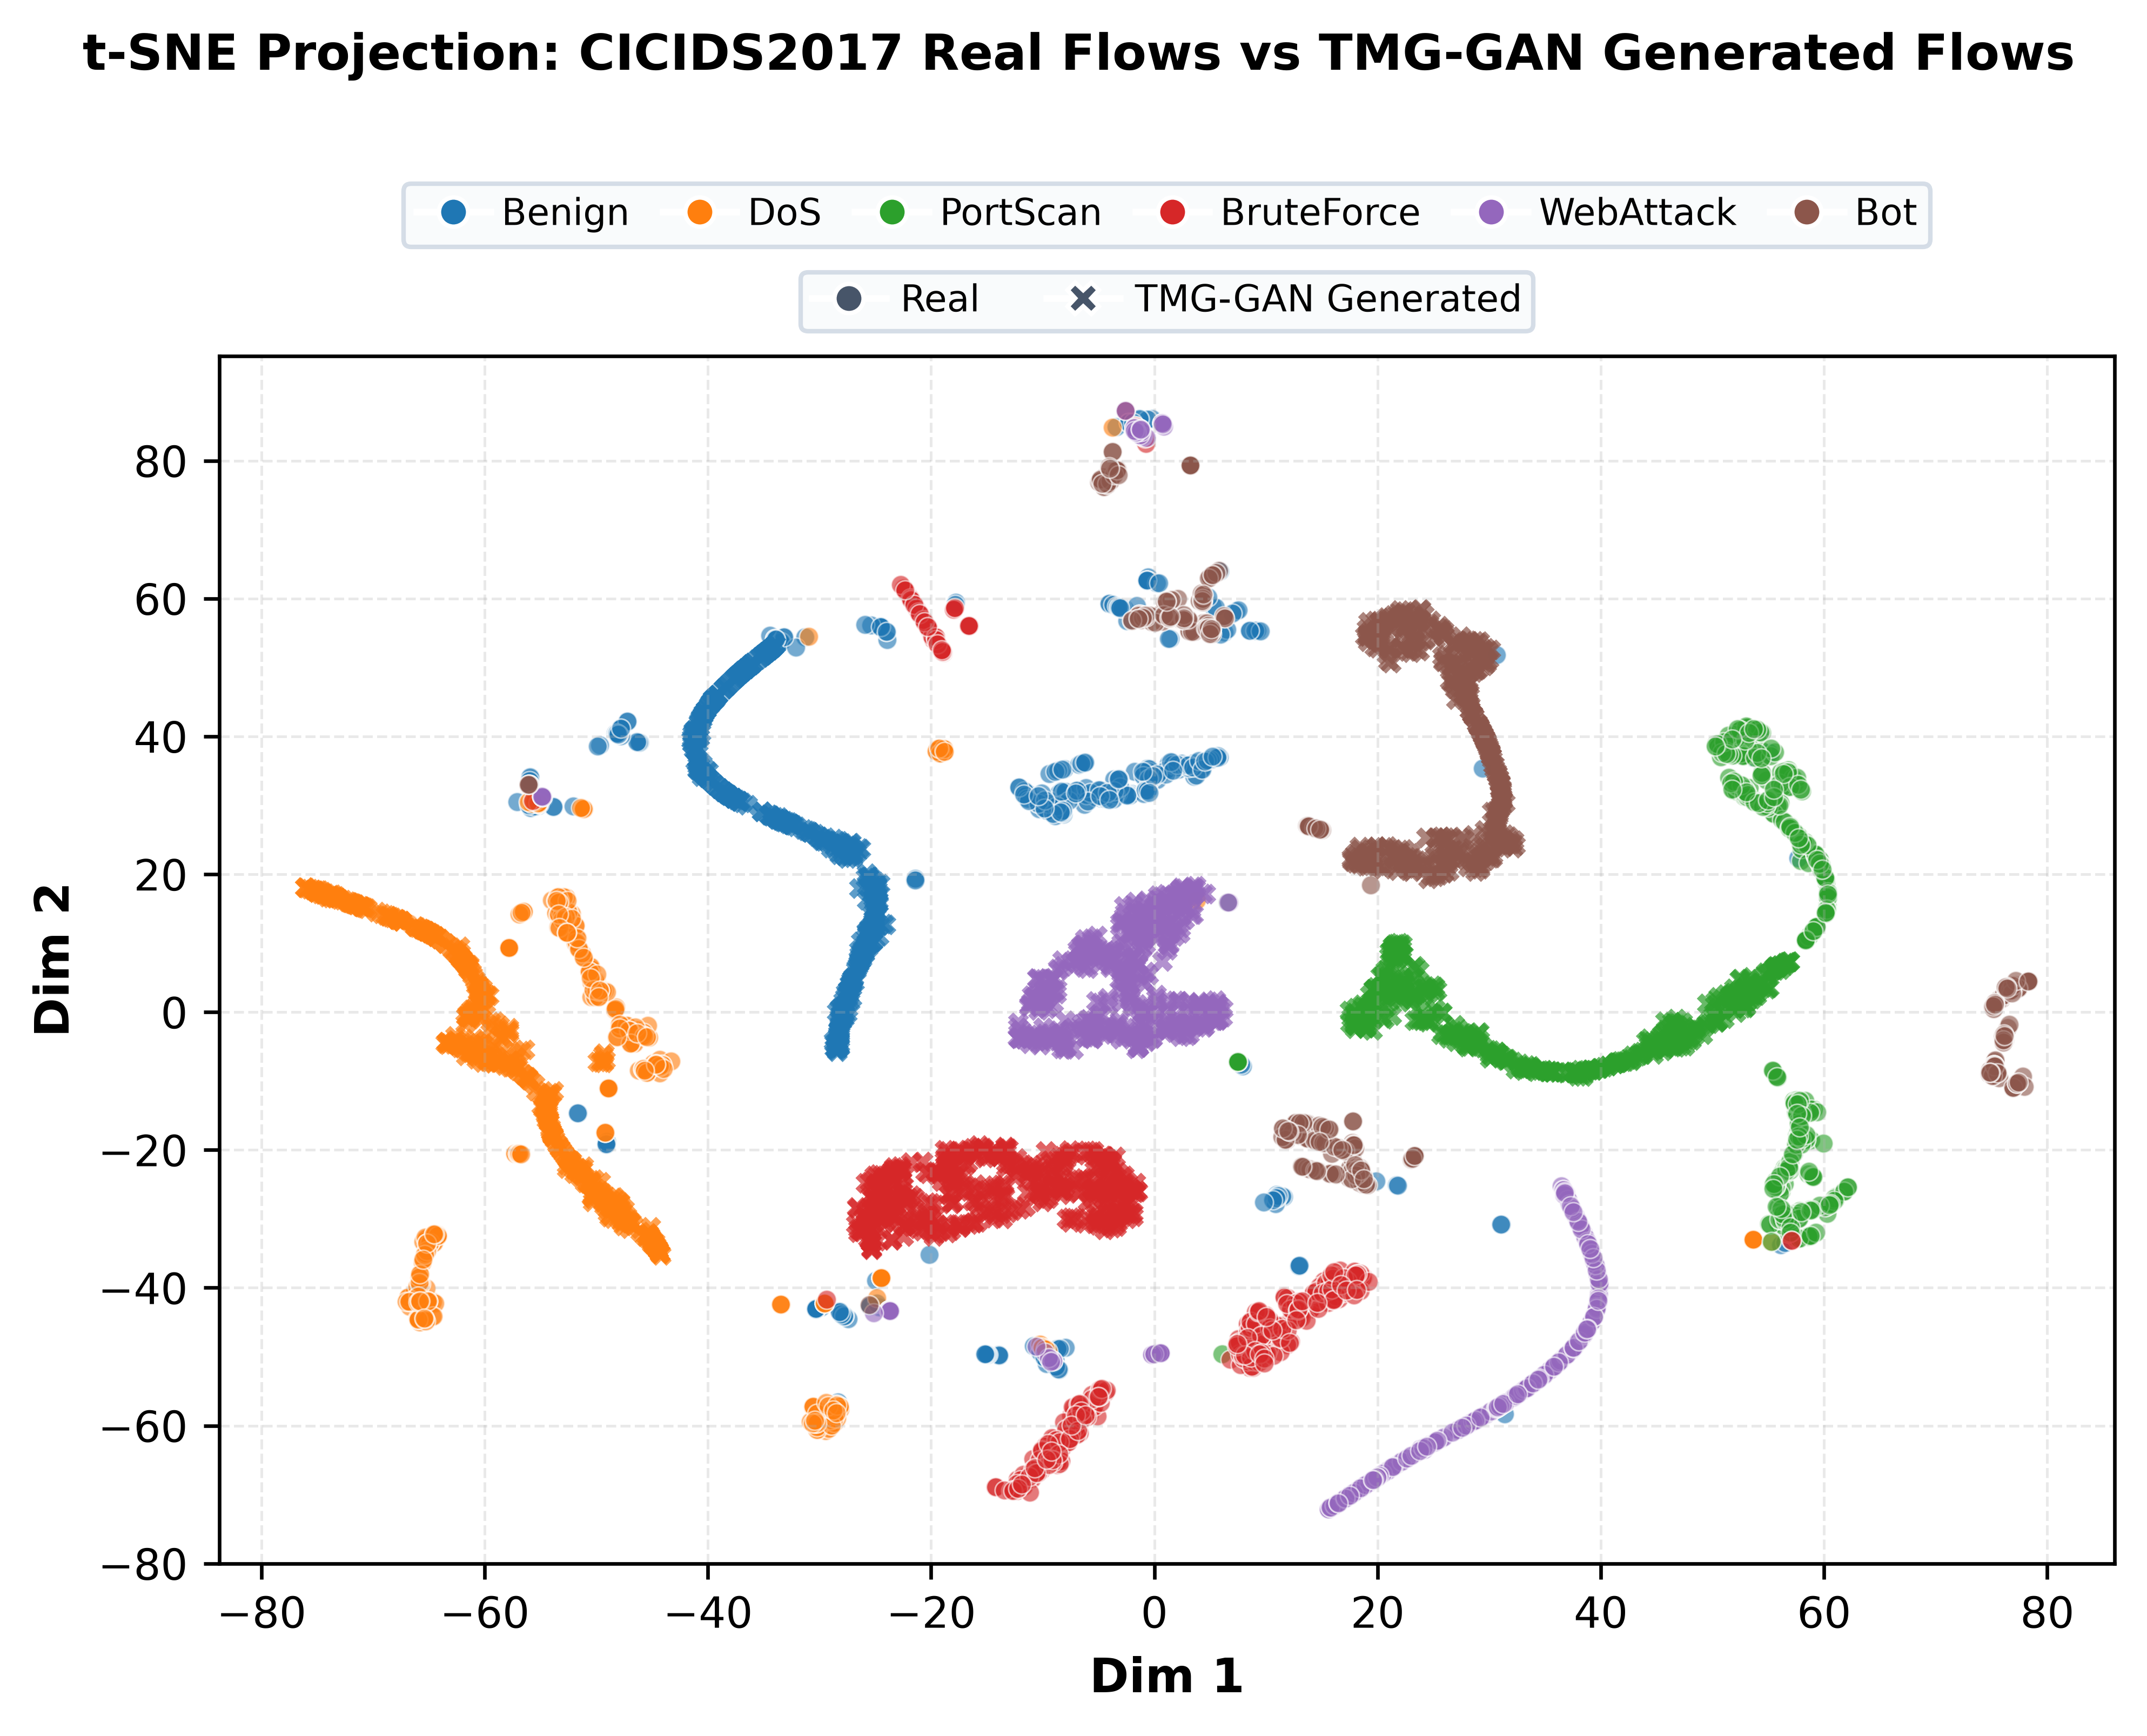
\includegraphics[width=\columnwidth]{figures/fig6_tsne_manifold.png}
\caption{Two-dimensional t-distributed stochastic neighbor embedding (t-SNE) projection of real versus synthetic feature representations across the five minority attack categories.}
\label{fig:tsne}
\end{figure}

To examine why DNN + TMG-GAN (Proposed) prevents boundary degradation, Fig.~\ref{fig:tsne} presents a two-dimensional t-SNE projection of real versus synthetic feature vectors. While linear interpolation scatters points across unpopulated feature space, the TMG-GAN generators produce synthetic flows clustered tightly along the true empirical attack distributions, preserving feature manifolds without invading benign decision regions.


\section{Conclusion and Future Work}

Network intrusion detection under severe class imbalance was investigated using the CICIDS2017 dataset. While SMOTE and ADASYN improve minority attack recall, linear interpolation produces artificial samples that pollute class boundaries, elevating the benign false-positive rate to $2.6366\%$ and $2.9324\%$. In contrast, the proposed TMG-GAN framework reshapes continuous statistics into $13 \times 6$ spatial matrices, decouples class-specific generation, and stabilizes adversarial training with spectral normalization and dual quality filtering. On 710,976 held-out test flows, TMG-GAN achieves a macro F1-score of $0.7940 \pm 0.0237$ and reduces the benign FPR to $2.3088\% \pm 0.2161\%$, eliminating over 2,038 false alarms compared to SMOTE and 3,877 false alarms compared to ADASYN. Future work will focus on optimizing the framework for FPGA-based inference and evaluating live 10~Gbps network traffic.

\bibliographystyle{IEEEtran}
\bibliography{references}

\end{document}
